\section{\color{magenta}Additional details on the numerical study\color{black}}\label{sec:supp:num_study}

\subsection{\color{magenta}Additional details on the simulation design\color{black}}

\begin{figure}[t!]
	\centering
	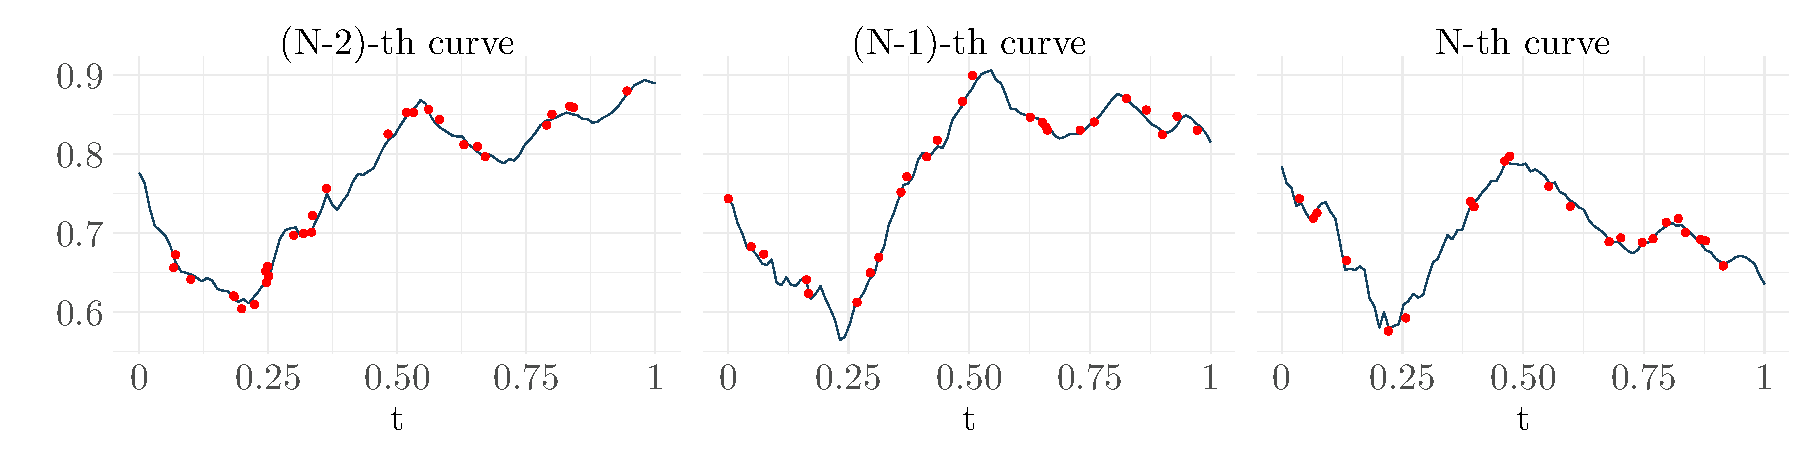
\includegraphics[width=\textwidth]{./figures/generated_conso_3last_curves.pdf}
	\caption{\small Last \color{magenta}three\color{black} simulated curves generated using the simulation setting with a sample size of $(N, \lambda) = (150, 25)$. The solid lines represent the sample paths, while the dots indicate the randomly observed noisy points on each curve, with an average of $\lambda = 25$ points per curve. \color{magenta}[TBC: the figure has been regenerated under the current design --- 10\_simulation\_design.R:464--465 draws curves $148$ to $150$ with \texttt{hurst\_linear(h\_left = 0.4, h\_right = 0.8)}, \texttt{intercept\_var = 0.05} and \texttt{sig\_obs = 0.007} --- but from the literal seed \texttt{12345} and with \texttt{L2 = 0.0107}, the mean of the estimates from the consumption curves (10\_simulation\_design.R:305), where the Monte Carlo of 11\_simulation\_generate.R:19 uses \texttt{L2 = 0.01}. Settle whether the illustration should instead be drawn from the Monte Carlo stream itself]\color{black}}
	\label{fig:generated_last_curves}
\end{figure}

\begin{figure}[h!]
	\centering
	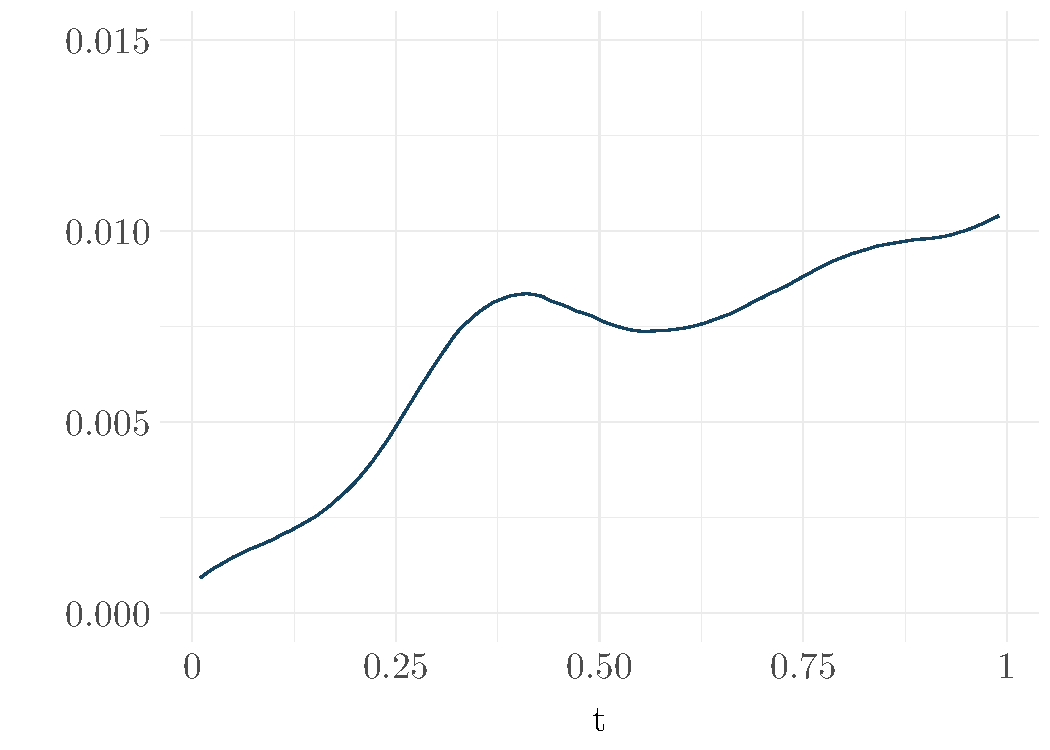
\includegraphics[width=0.4\textwidth]{./figures/variance_FTS_conso_lag=0.pdf}
	\caption{\small Variance of the constructed FTS process from \eqref{blup:FTS_mod1} and the consumption curves. \color{magenta}[TBC: the figure draws one line, not two. 30\_figures\_autocov.R:24--25 plots a single \texttt{geom\_line} of \texttt{autocovtilde} against $t$ from \texttt{dt\_true\_variance\_conso\_lag=0.RDS}, which 12\_simulation\_true\_autocov.R:83 forms on the simulated series alone; nothing of the consumption curves is drawn. Either drop ``and the consumption curves'' or add the second line]\color{black}}
	\label{fig:var_FTSConso}
\end{figure}

\subsection{Implementation details}

\subsubsection{\color{magenta}Adaptive (auto)covariance estimation\color{black}}

\color{magenta}
The estimation of the lag-$\ell$, $\ell \geq 0$, (auto)covariance using the estimators in [TBC: \texttt{eq:hat\_Gamma\_ell}, \texttt{eq:hat\_Gamma\_0:diagonal\_outside}, \texttt{eq:hat\_Gamma\_0:diagonal} --- labels not defined in best\_predictor\_aout24.tex] involves selecting optimal bandwidths based on the data-driven rules given in [TBC: \texttt{eq:gamma:risk-minimization}, \texttt{eq:gamma\_0:diagonal\_outside:risk-minimization}, \texttt{eq:gamma\_0\_diag:risk-minimization} --- labels not defined in best\_predictor\_aout24.tex], respectively. Computing $\widehat{R}_{c_\ell}$ requires estimating the dependence coefficients $\mathbb{D}_\ell(s, t; h_s, h_t)$, $\mathbb{D}_\ell(t,h_t|s,h_s)$, and $\mathbb{D}(t; h_t)$, which is computationally intensive.
To reduce computation time, we adopt a simplified approach. Let $\widetilde{X}_n$ denote the NW estimator of the curve $X_n$, obtained using a bandwidth selected via cross-validation. Given a set of sample points $\{(Y_{n,1}, T_{n,1}), \ldots, (Y_{n,M_n}, T_{n,M_n})\}$ for a curve $X_n$, the cross-validated optimal bandwidth for the estimator in [TBC: \texttt{eq:blup:LP\_est\_v} --- label not defined in best\_predictor\_aout24.tex] is defined as
\color{black}
\begin{equation}\label{eq:NW_bw_cv}
	h^* \in \argmin_h \sum_{i = 1}^{M_n}\left\{Y_{n,i} - \widetilde{X}_n^{(-i)}(T_{n,i};h)\right\}^2,
\end{equation}
\color{magenta}
where $\widetilde{X}_n^{(-i)}(T_{n,i};h)$ denotes the estimator in [TBC: \texttt{eq:blup:LP\_est\_v} --- label not defined in best\_predictor\_aout24.tex] computed without the $i$-th observation and using bandwidth $h$. \color{black}Moreover, let $\widetilde{Z}_n(t) = \widetilde{X}_n(t) - \widetilde{\mu}_N(t)$, and define, for all $s, t \in I$,
\begin{equation*}
	\widetilde{\mu}_N(t) = \frac{1}{N} \sum_{n=1}^{N} \widetilde{X}_{n}(t), \qquad
	\color{magenta}\widetilde{c}_\ell(s, t)\color{black} = \frac{1}{N - \ell} \sum_{n = 1}^{N - \ell} \widetilde{Z}_n(s) \widetilde{Z}_{n + \ell}(t), \quad \ell \geq 1.
\end{equation*}
Then, instead of estimating $\mathbb{D}_\ell(s, t; h_s, h_t)$, $\mathbb{D}_\ell(t,h_t|s,h_s)$, and $\mathbb{D}(t; h_t)$, we simply consider the following
\begin{multline}
	\widehat{\mathbb{D}}_\ell(s,t;h_s, h_t)
	= \frac{1}{N-\ell} \sum_{n=1}^{N - \ell} \left\{\widetilde{Z}_n(s) \widetilde{Z}_{n + \ell}(t) - \color{magenta}\widetilde{c}_\ell (s,t)\color{black}\right\}^2 \\
	+ \!\!\!\!\sum_{k = 1}^{N-\ell - 1}\frac{2 P_{N,\ell}^{-1}(s, t; h_s, h_t)}{N - \ell - k} \Biggl|\sum_{n = 1}^{N - \ell - k - 1}\!\left\{\widetilde{Z}_n(s) \widetilde{Z}_{n + \ell}(t) - \color{magenta}\widetilde{c}_\ell (s,t)\color{black}\right\} \left\{\widetilde{Z}_{n + k}(s) \widetilde{Z}_{n + \ell + k}(t) - \color{magenta}\widetilde{c}_\ell (s,t)\color{black}\right\}\!\Biggr|,
\end{multline}
\begin{multline}
	\widehat{\mathbb{D}}_\ell(t,h_t|s,h_s)  = 24 \!\!\!\!\!\!\!\!\!\!\!\!\!\!\!\!\!\sum_{1\leq n_1<n_2<n_3\leq \ell_{\max}}\!\!\!\!\!\!\!\!\!\!\!\!\!\!\!\!(N - n_3)^{-1}\left|\sum_{k=1}^{N - n_3} \!\! \frac{p_{k,n_1, n_2}(t;h_t)}{P_{N,\ell}^{3}(s, t; h_s, h_t)} \left\{\widetilde{Z}_k \widetilde{Z}_{k + n_1} \widetilde{Z}_{k + n_2} \widetilde{Z}_{k + n_3}\right\}(t) \right| \\
	+ 6 \!\!\!\!\!\!\!\!\!\!\!\!\!\!\sum_{1\leq n_1<n_2\leq \ell_{\max}} \!\!\!\!\!\!\!\!\!\!\!\!\!(N - n_2)^{-1}\left|\sum_{k=1}^{N - n_2} \! \frac{p_{k,n_1, n_2, n_3}(t;h_t)}{P_{N,\ell}^{3}(s, t; h_s, h_t)} \left\{\widetilde{Z}_k^2 \widetilde{Z}_{k + n_1} \widetilde{Z}_{k + n_2} + \widetilde{Z}_k \widetilde{Z}_{k + n_1}^2 \widetilde{Z}_{k + n_2} + \widetilde{Z}_k \widetilde{Z}_{k + n_1} \widetilde{Z}_{k + n_2}^2\right\}(t)\right|,
\end{multline}
\begin{multline}
	\widehat{\mathbb{D}}(t; h_t)  = 24 \!\!\!\!\!\!\!\!\!\!\!\!\!\!\!\!\!\sum_{1\leq n_1<n_2<n_3\leq \ell_{\max}}\!\!\!\!\!\!\!\!\!\!\!\!\!\!\!\!(N - n_3)^{-1}\left|\sum_{k=1}^{N - n_3} \!\! \frac{p_{k,n_1, n_2}(t;h_t)}{P_N^{3}(t; h_t)}\left\{\widetilde{Z}_k \widetilde{Z}_{k + n_1} \widetilde{Z}_{k + n_2} \widetilde{Z}_{k + n_3}\right\}(t) \right| \\
	+ 6 \!\!\!\!\!\!\!\!\!\!\!\!\!\!\sum_{1\leq n_1<n_2\leq \ell_{\max}} \!\!\!\!\!\!\!\!\!\!\!\!\!(N - n_2)^{-1}\left|\sum_{k=1}^{N - n_2} \!\frac{p_{k,n_1, n_2, n_3}(t;h_t)}{P_N^{3}(t; h_t)} \left\{\widetilde{Z}_k^2 \widetilde{Z}_{k + n_1} \widetilde{Z}_{k + n_2} + \widetilde{Z}_k \widetilde{Z}_{k + n_1}^2 \widetilde{Z}_{k + n_2} + \widetilde{Z}_k \widetilde{Z}_{k + n_1} \widetilde{Z}_{k + n_2}^2\right\}(t)\right|,
\end{multline}
where $N \gg \ell_{\max} = 3$ to avoid $\Oo(N^4)$ or $\Oo(N^3)$ complexity, and
\begin{align}
	p_{k,n_1, n_2}(t;h_t) &= \pi_k(t;h_t)\pi_{k+n_1}(t;h_t)\pi_{k+n_2}(t;h_t), \\
	p_{k,n_1, n_2, n_3}(t;h_t) &= \pi_k(t;h_t)\pi_{k+n_1}(t;h_t)\pi_{k+n_2}(t;h_t)\pi_{k+n_3}(t;h_t).
\end{align}

\color{magenta}
[TBC: $\widehat{R}_{c_\ell}$, $\mathbb{D}$, $\mathbb{B}$, $\mathbb{V}$, $P_N$, $P_{N,\ell}$ and $\pi_n$ are not attested in best\_predictor\_aout24.tex; the risk-bound apparatus they belong to is absent from it. Either it returns to the authority or this subsection must define what it uses]
\color{black}

\subsubsection{\color{magenta}Tikhonov parameter selection\color{black}}

\color{magenta}
[TBC: protocol, from adaptiveFTS \texttt{select\_tikhonov\_parameter} (R/11\_blup.R:329--453). One-step-ahead cross-validation over the last \texttt{n\_cv\_curves} curves; each target is predicted from its immediate predecessor and scored by \eqref{eq:weighted_ise} formed on that target, the weights being those of the held-out curve. Under the common design the operators are estimated once on the training block; under the independent design a rolling origin refreshes the plug-in estimates on all curves up to the predecessor, with bandwidths held at those selected on the initial block. Only the $M\times M$ system depends on $\alpha$, so one eigendecomposition per fold serves the whole grid. Selection is the grid minimiser of the mean score, with a warning at a grid boundary. The simulation grid is $\exp(\texttt{seq}(-16, 3, \texttt{length.out} = 40))$, 22\_simulation\_blup.R:70]
\color{black}

\subsubsection{\color{magenta}Design-density bandwidth selection\color{black}}

\color{magenta}
[TBC: protocol, from adaptiveFTS \texttt{get\_density\_optimal\_bw} (R/10\_density\_estimator.R:201--234). For each sampled curve the bandwidth minimising the least-squares cross-validation score of \texttt{estimate\_density} over the grid is computed, and the median of the per-curve optima is returned; the BLUP then reuses that single bandwidth for every curve, so the design weights are consistent across curves. The simulation grid is log-spaced from $1/\lambda$ to $1$ over 20 points, 22\_simulation\_blup.R:61--64. Not selected under the common design, where every point is weighted equally]
\color{black}

\subsection{\color{magenta}Local regularity estimation\color{black}}

\color{magenta}
[TBC: local regularity at four locations against the design's own $H_t$. Requires 25\_simulation\_locreg.R then 35\_figures\_locreg.R; data-simulation/estimates/ has no locreg/ directory and figures/locreg/ is empty]
\color{black}

\subsection{\color{magenta}Risk surfaces and bandwidth selection\color{black}}

\color{magenta}
In this section we give more details on the bandwidth selection of the adaptive (auto)covariance estimators introduced in the main manuscript. The estimator selects one bandwidth per argument, so what has to be shown is that the two are genuinely different, and that they differ by more the further apart the local regularities at the two arguments are.

To this end, we consider four pairs $(s, t)$ and compute the average of the lag-$1$ autocovariance risk function $\widehat{R}_{c_1}(s, t; h_s, h_t)$, as defined in [TBC: \texttt{eq:risk-Gamma} --- label not defined in best\_predictor\_aout24.tex], over a bandwidth grid $\Hh_N \times \Hh_N$ based on the $R = 400$ FTS replications. Figure~\ref{fig:autocov_risk_2bw} shows the mean of the $400$ replications of the estimates of the lag-$1$ autocovariance risk function for $(N, \lambda) = (150, 100)$ at four locations $(s,t)$. These plots provide evidence that the estimates of the risk function are a convex function of $(h_s, h_t)$ at all four pairs, so that each surface has one minimum to report.

The minima are the point of the figure. Since the regularity varies along the domain (see Figure~\ref{fig:simu_param}-(a)), as expected, the minimising pairs $(h_1^*(s|t), h_1^*(t|s))$ are reached such that $h_1^*(s|t) \neq h_1^*(t|s)$ when $H_s \neq H_t$. Read in order of $|H_s - H_t|$, the four minima are $(0.00971, 0.00971)$ at $(0.7, 0.8)$, $(0.00427, 0.00738)$ at $(0.2, 0.4)$, $(0.00561, 0.00971)$ at $(0.4, 0.7)$ and $(0.01276, 0.00427)$ at $(0.8, 0.2)$; the ratio of the larger bandwidth to the smaller runs $1.00$, $1.73$, $1.73$ and $2.99$. The difference between the selected bandwidths is therefore greater for pairs $(s,t)$ such that $|H_s - H_t|$ is large, the two intermediate pairs being tied at this sample size.

At $(0.7, 0.8)$ the two bandwidths coincide. That is the rule working rather than failing: with the two regularities as close as the four pairs allow, there is nothing for two bandwidths to separate over, and the minimum of the surface falls on the diagonal $h_s = h_t$. As a consequence the figure carries both halves of the claim, the separation and its absence, on the same four panels.
\color{black}

\begin{figure}[h!]
	\centering
	\begin{tabular}{cc}
		\color{magenta}$(s, t)= (0.2, 0.4)$\color{black} & \color{magenta}$(s, t)= (0.4, 0.7)$\color{black}\\
		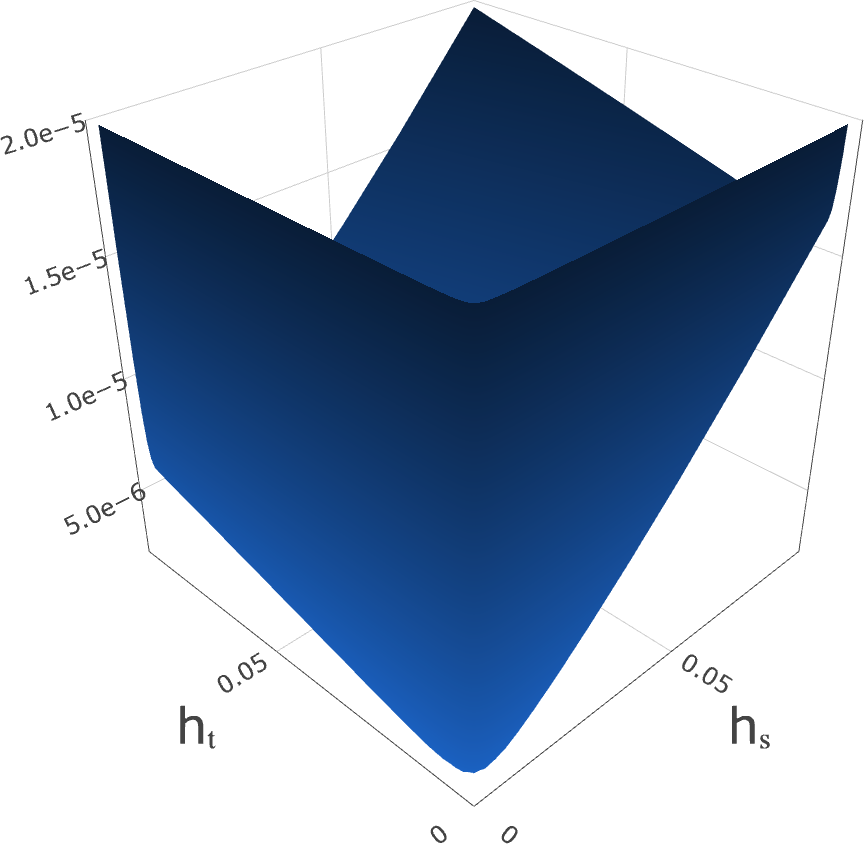
\includegraphics[width=0.35\textwidth]{./figures/autocov/plt_autocov_risk_conso_design_N=150_lambda=100_s=0.2_t=0.4.png} & 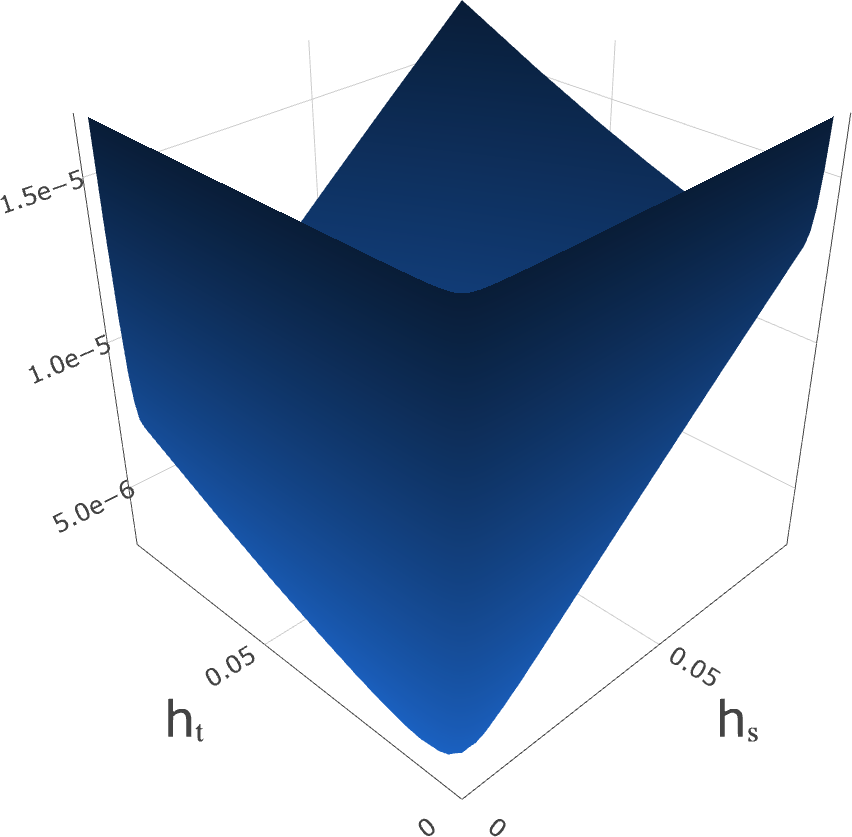
\includegraphics[width=0.35\textwidth]{./figures/autocov/plt_autocov_risk_conso_design_N=150_lambda=100_s=0.4_t=0.7.png}\\
		\color{magenta}$(H_s, H_t) = (0.48, 0.56)$\color{black} & \color{magenta}$(H_s, H_t) = (0.56, 0.68)$\color{black}\\
		\color{magenta}$(h_1^*(s|t), h_1^*(t|s)) = (0.00427, 0.00738)$\color{black} & \color{magenta}$(h_1^*(s|t), h_1^*(t|s)) = (0.00561, 0.00971)$\color{black} \\
		& \\
		& \\
		\color{magenta}$(s, t)= (0.7, 0.8)$\color{black} & \color{magenta}$(s, t)= (0.8, 0.2)$\color{black}\\
		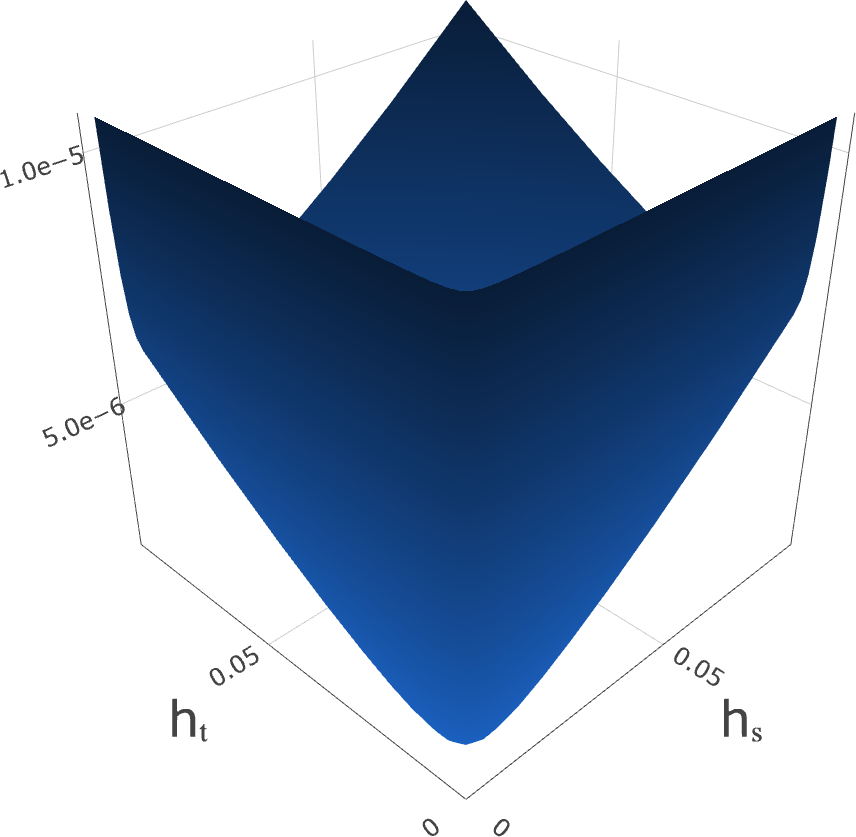
\includegraphics[width=0.35\textwidth]{./figures/autocov/plt_autocov_risk_conso_design_N=150_lambda=100_s=0.7_t=0.8.png} &
		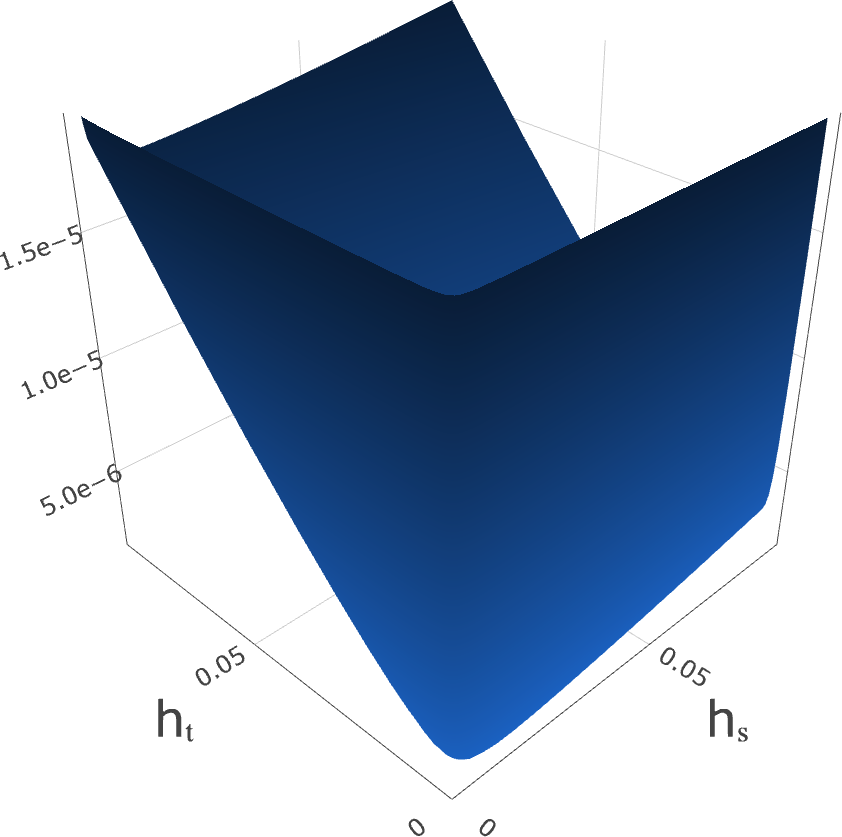
\includegraphics[width=0.35\textwidth]{./figures/autocov/plt_autocov_risk_conso_design_N=150_lambda=100_s=0.8_t=0.2.png}\\
		\color{magenta}$(H_s, H_t) = (0.68, 0.72)$\color{black} & \color{magenta}$(H_s, H_t) = (0.72, 0.48)$\color{black}\\
		\color{magenta}$(h_1^*(s|t), h_1^*(t|s)) = (0.00971, 0.00971)$\color{black} & \color{magenta}$(h_1^*(s|t), h_1^*(t|s)) = (0.01276, 0.00427)$\color{black}
	\end{tabular}
	\caption{\small Empirical average of the risk function \color{magenta}$\widehat{R}_{c_1}(s,t;h_s, h_t)$\color{black} at \color{magenta}$(s,t) \in \{ (0.2, 0.4)$, $(0.4, 0.7)$, $(0.7, 0.8)$, $(0.8, 0.2)\}$\color{black} computed over $400$ independent replications of the FTS for the sample size $(N, \lambda) = (150, 100)$. \color{magenta}Each panel is headed by its pair $(s,t)$. Beneath the surface are the two local Hölder exponents at that pair and, on the last line, the bandwidth pair $(h_1^*(s|t), h_1^*(t|s))$ at which the plotted surface attains its minimum. The two horizontal axes of a surface are $h_s$ and $h_t$ and the vertical axis is the risk; the surfaces are windowed to bandwidths no greater than $0.09$.\color{black}}
	\label{fig:autocov_risk_2bw}
\end{figure}

\color{magenta}
Our new adaptive covariance estimator involves selecting optimal bandwidths by minimising both the estimates of the bivariate risk function [TBC: \texttt{eq:risk-Gamma\_0:diagonal\_outside} --- label not defined in best\_predictor\_aout24.tex] outside the diagonal band and the estimates of the univariate risk function given in [TBC: \texttt{eq:risk-Gamma\_0} --- label not defined in best\_predictor\_aout24.tex] for the diagonal line estimator. We consider the same setups and generated data as in the autocovariance estimation study to illustrate the performance of our new covariance estimator.
\color{black}

\color{magenta}
First, regarding the risk function estimation, Figure~\ref{fig:cov_risk_2bw} shows the average over the $400$ replications of the estimates of the covariance risk function [TBC: \texttt{eq:risk-Gamma\_0:diagonal\_outside} --- label not defined in best\_predictor\_aout24.tex] for $(N, \lambda) = (150, 100)$ at the same four locations. These plots provide evidence that the risk function is convex and can thus be effectively minimised to obtain optimal bandwidth pairs. Similarly, Figure~\ref{fig:diagonal_risk} illustrates that the risk function for the diagonal line is also convex, allowing straightforward selection of the optimal bandwidth for its estimation.
\color{black}

\color{magenta}
Furthermore, for the bivariate risk function [TBC: \texttt{eq:risk-Gamma\_0:diagonal\_outside} --- label not defined in best\_predictor\_aout24.tex], since the regularity varies across the domain (see Figure~\ref{fig:simu_param}-(a)), the optimal bandwidth pairs $(h_0^*(s|t), h_0^*(t|s))$ are again such that $h_0^*(s|t) \neq h_0^*(t|s)$ when $H_s \neq H_t$. Read in order of $|H_s - H_t|$, the four minima are $(0.01276, 0.01276)$ at $(0.7, 0.8)$, $(0.00561, 0.00738)$ at $(0.2, 0.4)$, $(0.00561, 0.01276)$ at $(0.4, 0.7)$ and $(0.01276, 0.00427)$ at $(0.8, 0.2)$; the ratio of the larger bandwidth to the smaller runs $1.00$, $1.31$, $2.27$ and $2.99$. The difference between the selected bandwidths therefore grows at every step with the difference in local regularity, and at $(0.7, 0.8)$, where that difference is smallest, it does not exist at all: both bandwidths are $0.01276$.

The bandwidths selected at lag $0$ are wider than their lag-$1$ counterparts at three of the four pairs. This ordering of the selected bandwidths is not inherited by the accuracy of the estimator: the error ratios reported in the main manuscript separate the four pairs much less clearly at lag $0$ than at lag $1$.
\color{black}

\begin{figure}[h!]
		\centering
	\begin{tabular}{cc}
		\color{magenta}$(s, t)= (0.2, 0.4)$\color{black} & \color{magenta}$(s, t)= (0.4, 0.7)$\color{black}\\
		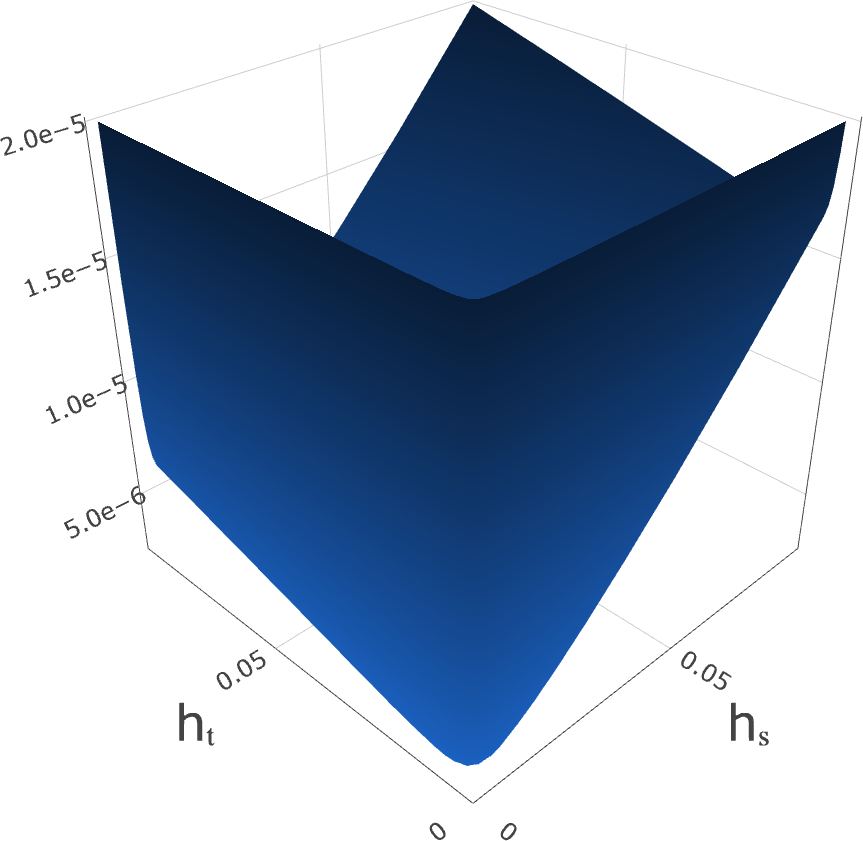
\includegraphics[width=0.35\textwidth]{./figures/cov/plt_cov_risk_conso_design_N=150_lambda=100_s=0.2_t=0.4.png} & 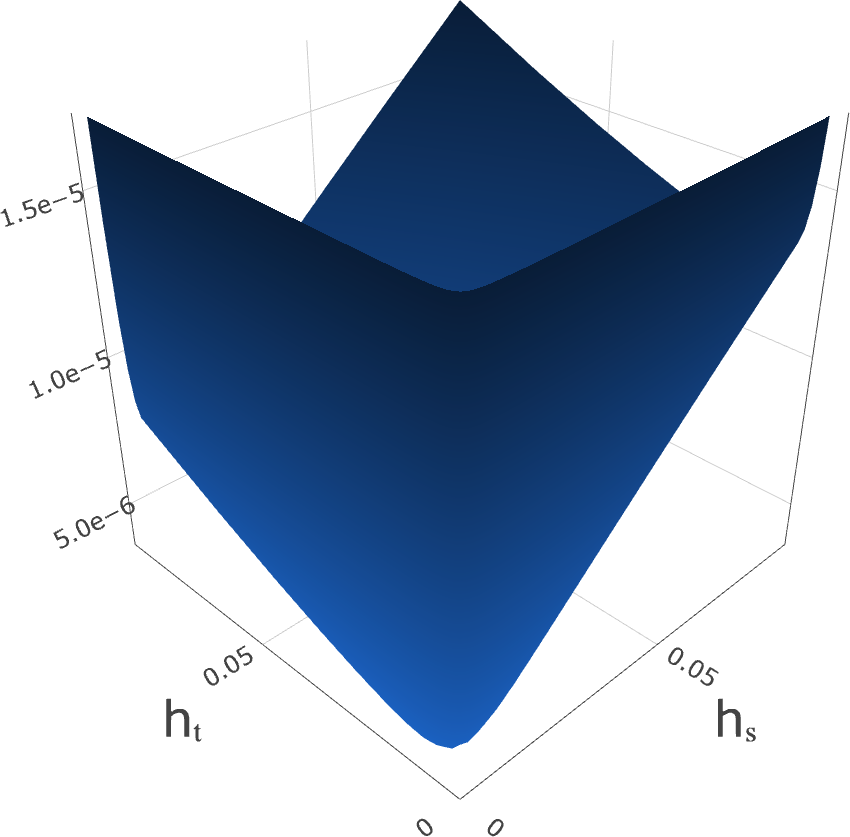
\includegraphics[width=0.35\textwidth]{./figures/cov/plt_cov_risk_conso_design_N=150_lambda=100_s=0.4_t=0.7.png}\\
		\color{magenta}$(H_s, H_t) = (0.48, 0.56)$\color{black} & \color{magenta}$(H_s, H_t) = (0.56, 0.68)$\color{black}\\
		\color{magenta}$(h_0^*(s|t), h_0^*(t|s)) = (0.00561, 0.00738)$\color{black} & \color{magenta}$(h_0^*(s|t), h_0^*(t|s)) = (0.00561, 0.01276)$\color{black} \\
		& \\
		& \\
		\color{magenta}$(s, t)= (0.7, 0.8)$\color{black} & \color{magenta}$(s, t)= (0.8, 0.2)$\color{black}\\
		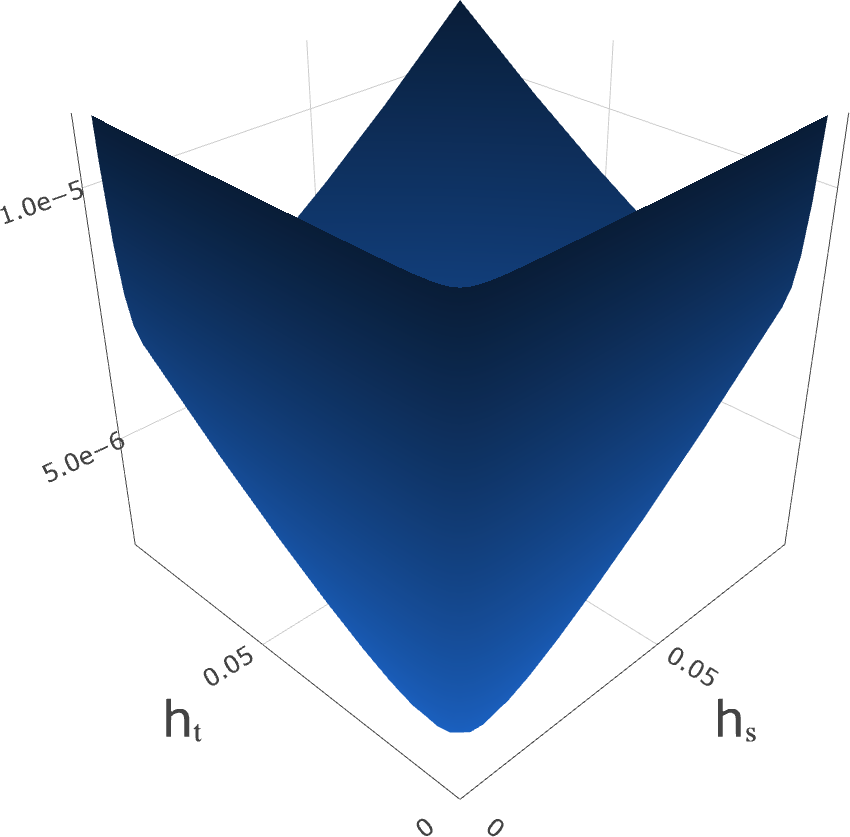
\includegraphics[width=0.35\textwidth]{./figures/cov/plt_cov_risk_conso_design_N=150_lambda=100_s=0.7_t=0.8.png} &
		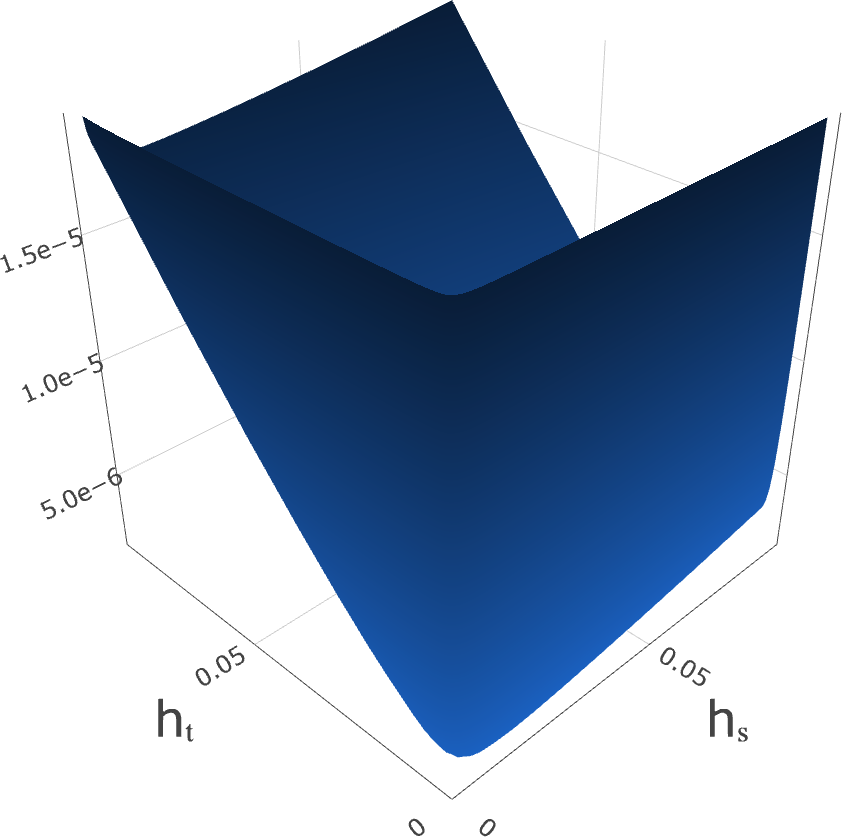
\includegraphics[width=0.35\textwidth]{./figures/cov/plt_cov_risk_conso_design_N=150_lambda=100_s=0.8_t=0.2.png}\\
		\color{magenta}$(H_s, H_t) = (0.68, 0.72)$\color{black} & \color{magenta}$(H_s, H_t) = (0.72, 0.48)$\color{black}\\
		\color{magenta}$(h_0^*(s|t), h_0^*(t|s)) = (0.01276, 0.01276)$\color{black} & \color{magenta}$(h_0^*(s|t), h_0^*(t|s)) = (0.01276, 0.00427)$\color{black}
	\end{tabular}
	\caption{\small Empirical average of the risk function \color{magenta}$\widehat{R}_{c_0}(s,t;h_s, h_t)$\color{black} at \color{magenta}$(s,t) \in \{ (0.2, 0.4)$, $(0.4, 0.7)$, $(0.7, 0.8)$, $(0.8, 0.2)\}$\color{black} computed over $400$ independent replications of the FTS for the sample size $(N, \lambda) = (150, 100)$. \color{magenta}The panels, the two annotation lines beneath each surface and the windowing of the bandwidths are those of Figure~\ref{fig:autocov_risk_2bw}, with $(h_0^*(s|t), h_0^*(t|s))$ in place of the lag-$1$ pair.\color{black}}
	\label{fig:cov_risk_2bw}
\end{figure}

\begin{figure}[th]
	\vspace{.1cm}
	\centering
	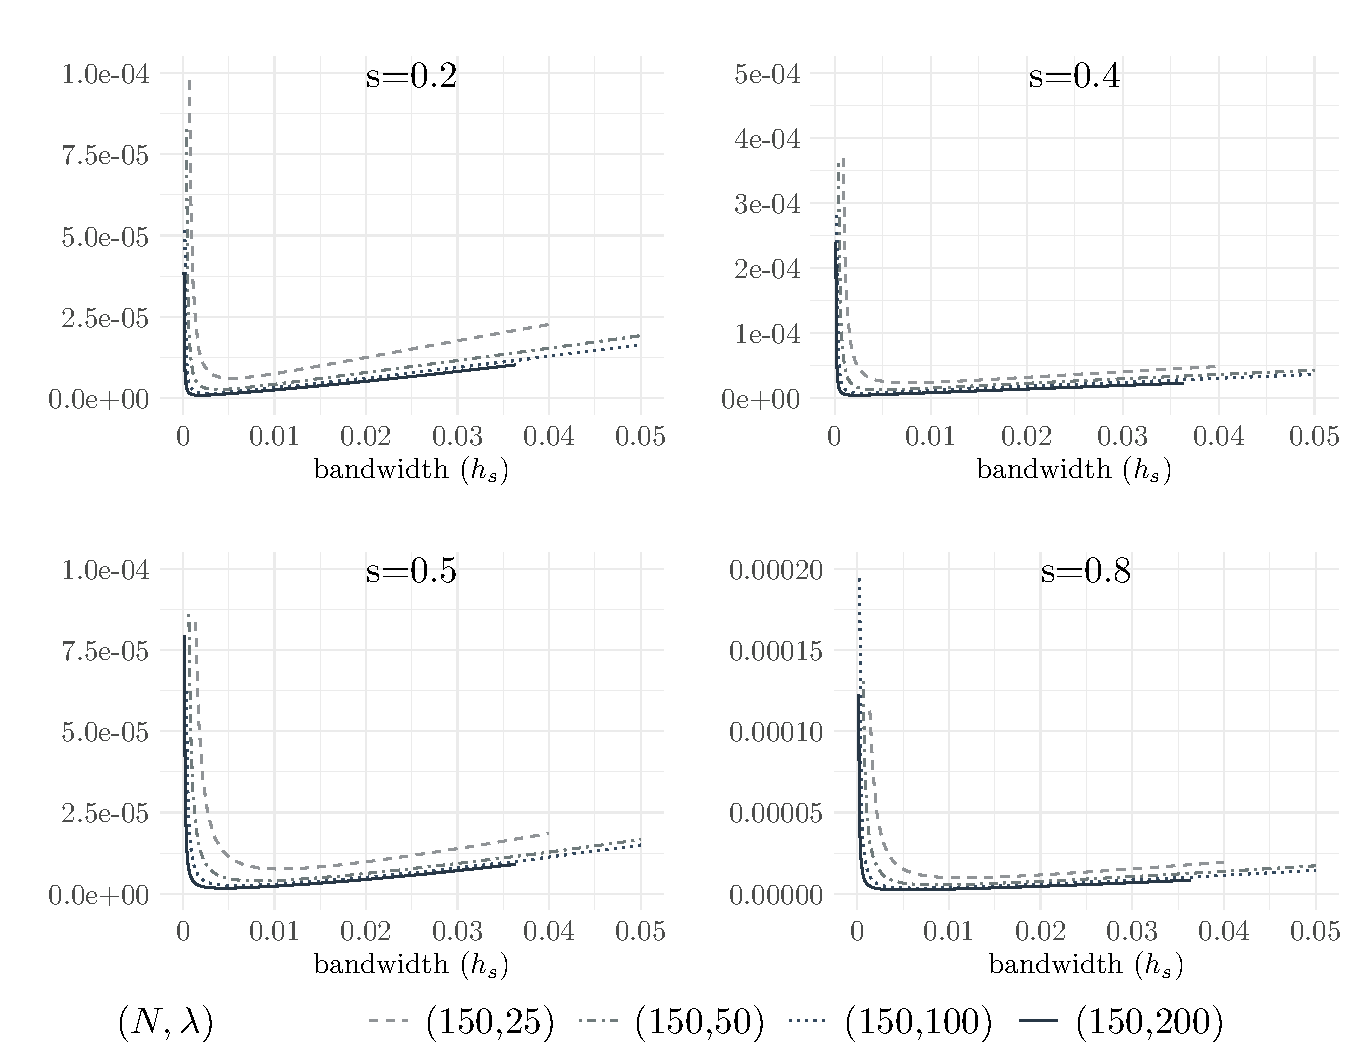
\includegraphics[width=0.9\linewidth]{./figures/cov/plt_diag_cov_risk_conso_N=150_all_lambda_all_4locations.pdf}
	\caption{\small Empirical average of the risk function $\widehat{R}_\mu(s, h_s)$ at $s \in \{0.2, 0.4, 0.5, 0.8\}$, computed over $400$ independent replications of the FTS for sample sizes $(N, \lambda) \in \{(150, 25), (150, 50), (150, 100), (150, 200)\}$.}
	\label{fig:diagonal_risk}
\end{figure}

\subsection{\color{magenta}Additional details on adaptive curve prediction\color{black}}

\subsubsection{Empirical autoregressive effect}

\color{magenta}
We use the same generated sample of FTS as in the study of the autocovariance function, estimate the lag-$1$ FACF for each of the $400$ FTS replications using \eqref{eq:blup:facf}, and display the resulting histograms in Figure~\ref{fig:conso_lag1_facf} for different sample sizes $(N, \lambda)$. The plots provide empirical evidence that the autocovariance-related blocks in $\VV_{n_0}$ are not nil. Moreover, for our simulated FAR(1) model, most of the lag-$1$ FACF values are concentrated between $0.2$ and $0.4$.
[TBC: notation superseded, needs review --- $\VV_{n_0}$ as in the main text. The quoted range $0.2$ to $0.4$ is unverified: 23\_simulation\_facf.R has not been run and data-simulation/estimates/ has no facf/ directory]
\color{black}

\begin{figure}[h]
	\centering
	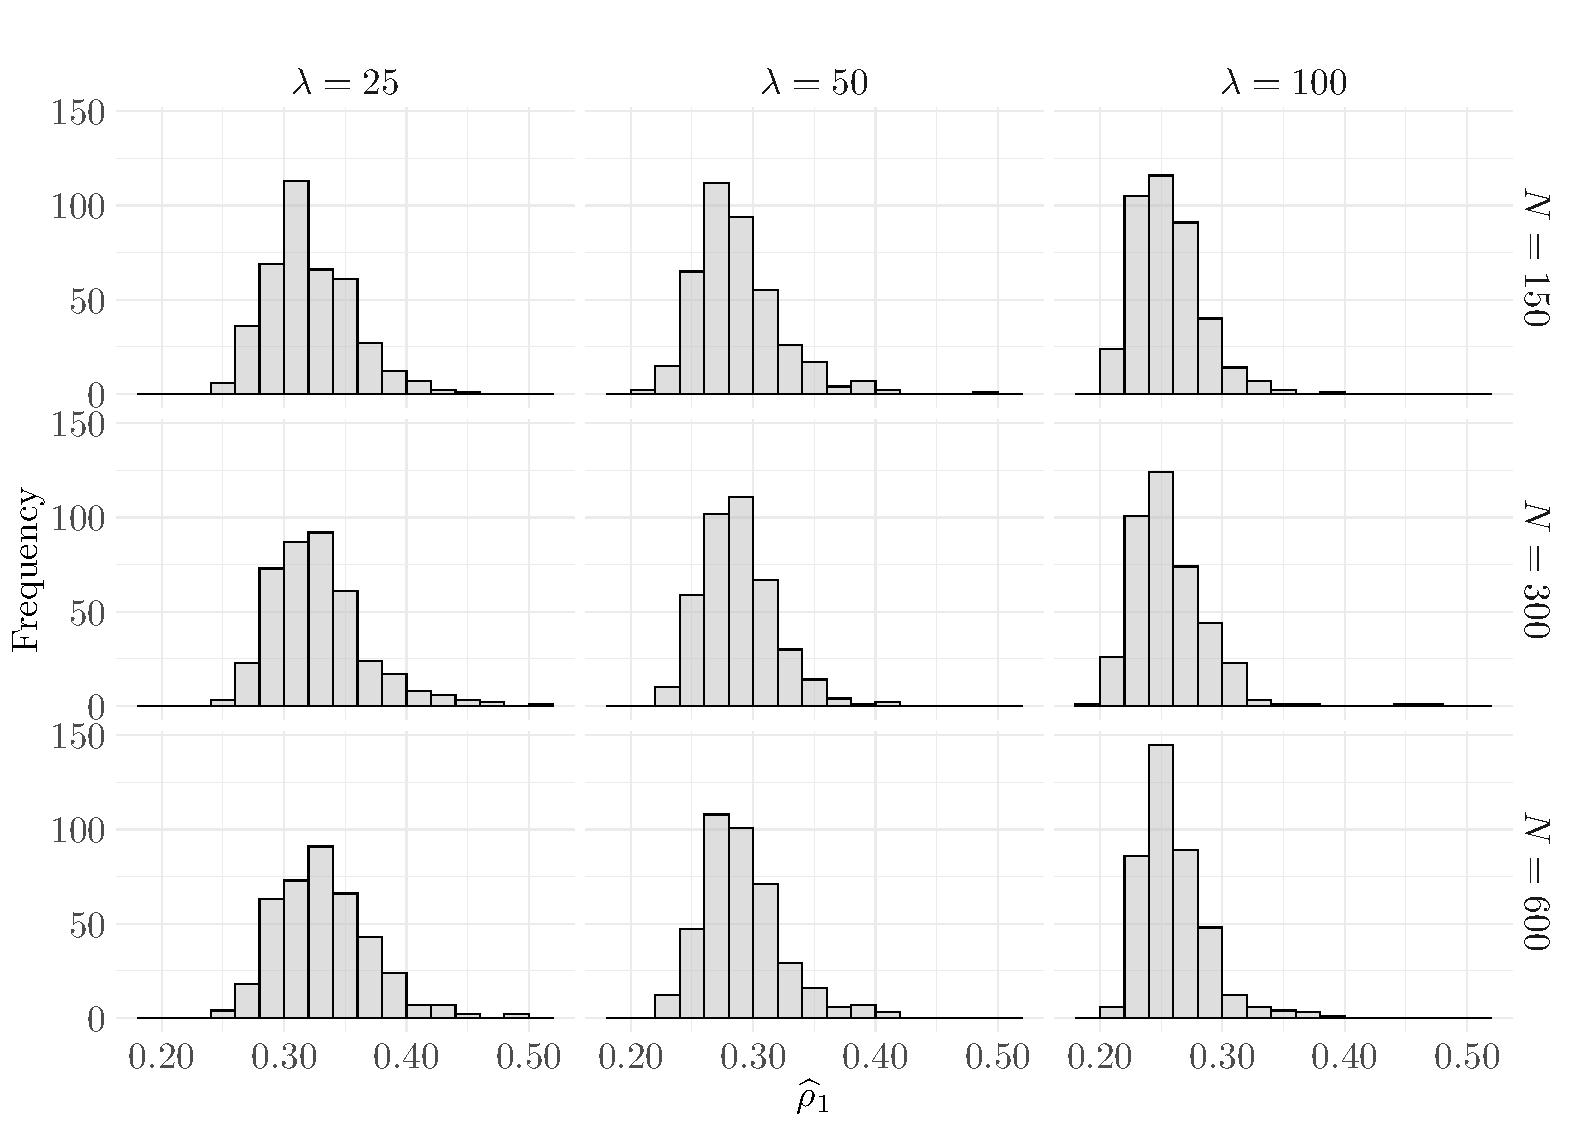
\includegraphics[width=\textwidth]{./figures/blup/hist_lag-1_facf_conso.pdf}
	\caption{\small Histograms of estimated lag-$1$ FACF values for different $(N, \lambda)$ configurations. \color{magenta}[TBC: the figure is a $3\times3$ grid, not the twelve setups of the study. 36\_figures\_facf.R:25 sets \texttt{lambdavec <- c(25, 50, 100)}, so $\lambda = 200$ is absent; :44--46 also pool every panel onto one set of Sturges breaks taken from the pooled values. Either restore $\lambda = 200$ in the script or say here which configurations are shown]\color{black}}
	\label{fig:conso_lag1_facf}
\end{figure}

\subsubsection{\color{magenta}Per-replication predicted curves\color{black}}

\color{magenta}
[TBC: four replications per sample size, true curve against adaptive prediction, both designs. Written by 32\_figures\_blup.R:206--267 as \texttt{plot\_blup\_mc\_conso\_N=*\_lambda=*} with a \texttt{\_common} suffix for the common design; figures/blup/ is empty]
\color{black}

\subsection{\color{magenta}Additional details on the real data applications\color{black}}

\subsubsection{\color{magenta}NOTPERP intraday volume\color{black}}

\color{magenta}
In this section we give more details on the NOTPERP volume application of the main manuscript, and in particular on the three preprocessing steps it names without describing. The trade archive of the ByBit exchange holds one compressed file per UTC calendar day; the $712$ files on disk cover 18 September 2024 to 30 August 2026 without a gap, and carry $1\,107\,894$ trades in all, from $132$ to $49\,768$ on a single day.

The mean function is constant in $n$ under our model, and the daily level of this series is not: the token was listed in September 2024 and its liquidity has declined since, a decline over which a linear trend accounts for $0.093$ of the variation of the daily total notional in logarithms. Rather than fix a period by hand, we retain the longest run of days ending at the last one over which a KPSS test does not reject a level null at the $5$ per cent level. That run is the $430$ days beginning 27 June 2025, over which the same linear trend accounts for $0.027$ of the variation. An augmented Dickey--Fuller test rejects a unit root on every window tried, so what the restriction removes is a drift and not an integrated level. The window is re-selected whenever the application is run, and therefore moves as the archive grows.

Outlying curves are then removed by an iterative functional boxplot based on the modified band depth. Functional depth requires a common grid, so for this step alone the curves are aggregated onto an equidistant grid of $\operatorname{median}_n M_n = 828$ points, each bin taking the last value observed within it; the value of a cumulative curve on a bin is the one it has reached by the end of it, and an average would report a value the curve never takes. At each round the curves lying beyond $1.5$ times the $50$ per cent central region are removed and the procedure is repeated. Round $1$ removed six curves, rounds $2$ and $3$ detected none, and the procedure terminated, leaving $N = 424$. Figure~\ref{fig:notperp_volume_fbplot} shows the boxplot at each round.

Two further steps make the sample the predictor is fitted on. About $14.4$ per cent of the rows share a timestamp with another, one market order filling against several resting ones, and the design times within a curve have to be distinct. The last row of each tied group is kept, which for a cumulative response is not an arbitrary choice: any earlier row of the group holds a partial sum, a value the curve takes at no instant at all. The number of observations per curve is then capped at $200$ by a uniform draw among the instants that remain, and $408$ of the $424$ curves sit on that cap. The cap is what makes the application tractable, the (auto)covariance estimators summing over the within-curve pairs of design points so that their cost grows about as $M_n^4$. It costs nothing here: the draw leaves the retained times an independent sample from the same design density, and each retained instant still carries the cumulative value realised at it, the cumulative sum being formed over every trade before anything is dropped.

The design density of \eqref{PR_weights} needs a bandwidth, and it is selected by cross-validation over $50$ curves drawn at random from the sample. The least-squares criterion for a density is unbounded as $h \to 0$, so it returns the lower edge of whatever grid it is given, and widening the grid only moves the answer. The grid is therefore floored at $1/\operatorname{median}_n M_n$, the mean spacing of the design, below which no bandwidth is admissible; the selection is the median of the per-curve optima and equals $0.005$, which is that floor, and nine tenths of the fifty curves attain their own optimum there. As a consequence this bandwidth is a property of the design rather than of the grid, and it is the one tuning parameter of the application that the data do not choose in the interior. Figure~\ref{fig:notperp_volume_cv} shows that criterion beside the Tikhonov criterion, whose minimum is interior.

Figure~\ref{fig:notperp_volume_locreg} presents the estimated local Hölder exponent and constant, evaluated at $99$ equally spaced points and smoothed by a cubic spline for display. The exponent runs from $0.254$ to $1$ with a median of $0.806$ and attains the upper end of the interval to which the estimator is clamped at $29$ of the $99$ points; the constant runs from $0.195$ to $28.8$. What these estimates support is the level of the exponent and not its variation across the domain, the estimator being known to shrink a varying exponent towards a narrow band. Figure~\ref{fig:notperp_volume_mean} presents the estimated mean function, which rises across the day as a cumulative response must.
[TBC: the functional boxplots of Figure~\ref{fig:notperp_volume_fbplot} are current, but Figures~\ref{fig:notperp_volume_cv}, \ref{fig:notperp_volume_locreg} and \ref{fig:notperp_volume_mean} were produced on 2026-08-31 between 00:56 and 01:24, before data-NOTPERP/raw/dt\_NOTPERP\_volume\_fts\_cleaned.csv was rewritten at 13:44 the same day. They inherit the flag raised in the main manuscript and must be regenerated by 46\_app\_notperp\_volume.R from the same run as the estimates]

[TBC: the modified band depth and the functional boxplot are due to a reference the bibliography does not carry. Add \texttt{roahd2019} --- Ieva, Paganoni, Romo and Tarabelloni, \emph{The R Journal} 11(2), 291--307, 2019 --- to references\_clean.bib, where it is present in paper\_for\_reference/NOTPERP\_descriptive\_analysis/report/references.bib:53, and cite it at the functional boxplot above]
\color{black}

\begin{figure}[h!]
	\centering
	\begin{tabular}{ccc}
		\color{magenta}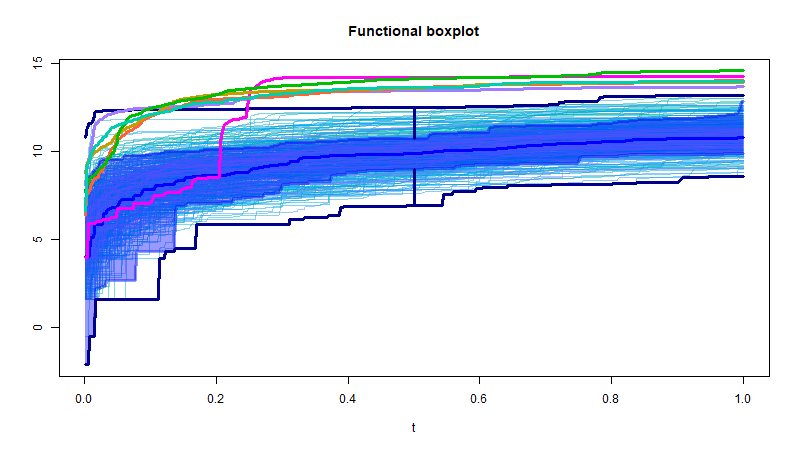
\includegraphics[width=0.31\textwidth]{./figures/notperp/Fboxplot_volume_round_1.png}\color{black} &
		\color{magenta}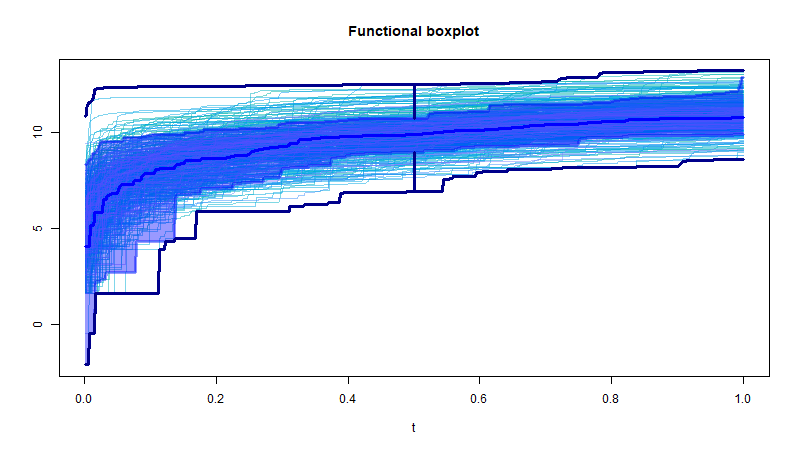
\includegraphics[width=0.31\textwidth]{./figures/notperp/Fboxplot_volume_round_2.png}\color{black} &
		\color{magenta}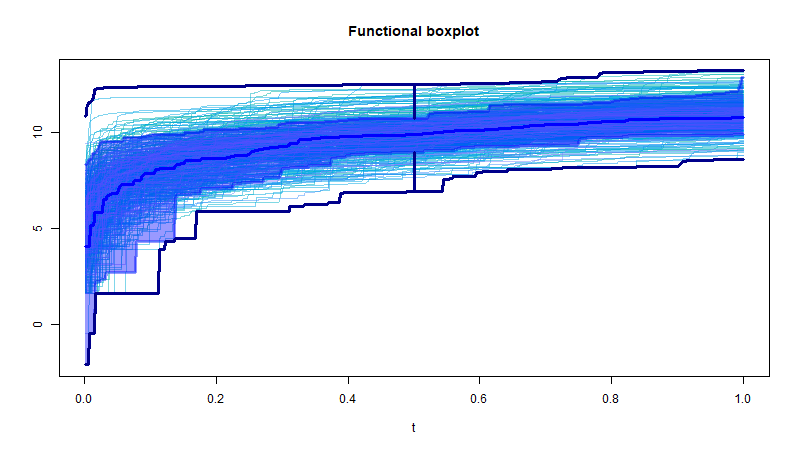
\includegraphics[width=0.31\textwidth]{./figures/notperp/Fboxplot_volume_round_3.png}\color{black}
	\end{tabular}
	\caption{\small \color{magenta}Iterative functional boxplot of the NOTPERP volume curves, based on the modified band depth and computed on the equidistant grid of $828$ points onto which the curves are aggregated for this step. \textbf{Left:} round $1$, on all $430$ curves of the stationary window, six outliers detected. \textbf{Middle:} round $2$, after their removal, none detected. \textbf{Right:} round $3$, none detected, and the procedure terminates. The shaded band is the $50$ per cent central region and the outlying curves are drawn apart from the rest.\color{black}}
	\label{fig:notperp_volume_fbplot}
\end{figure}

\begin{figure}[h!]
	\centering
	\begin{tabular}{cc}
		\color{magenta}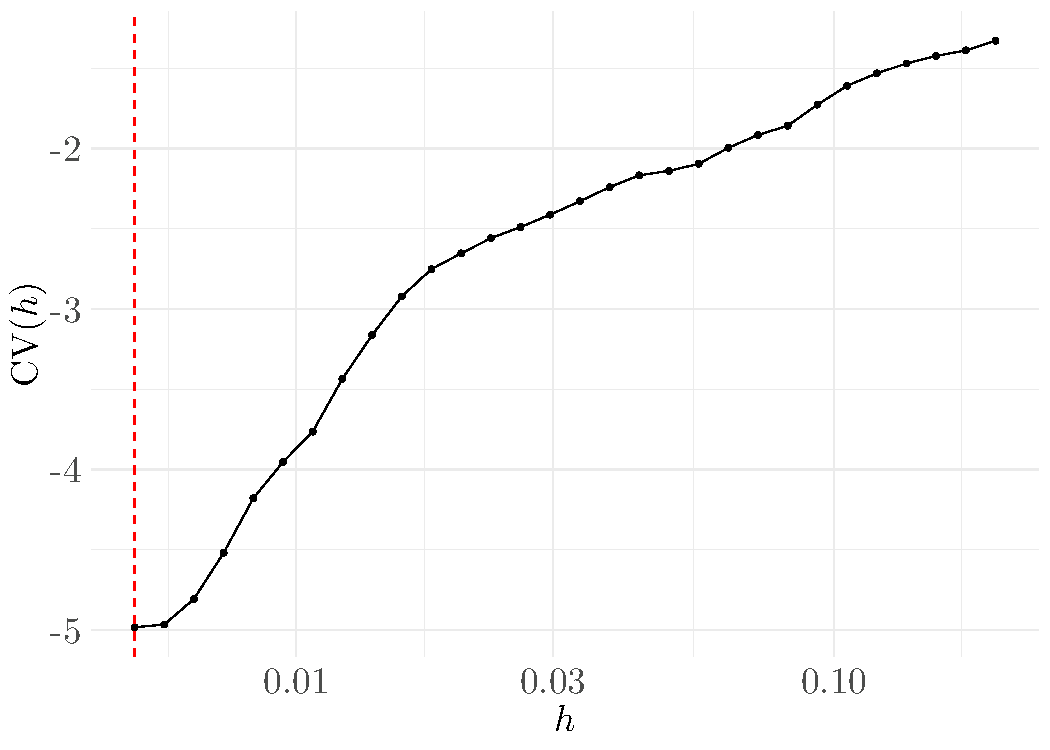
\includegraphics[width=0.45\textwidth]{./figures/notperp/NOTPERP_volume_density_cv.pdf}\color{black} &
		\color{magenta}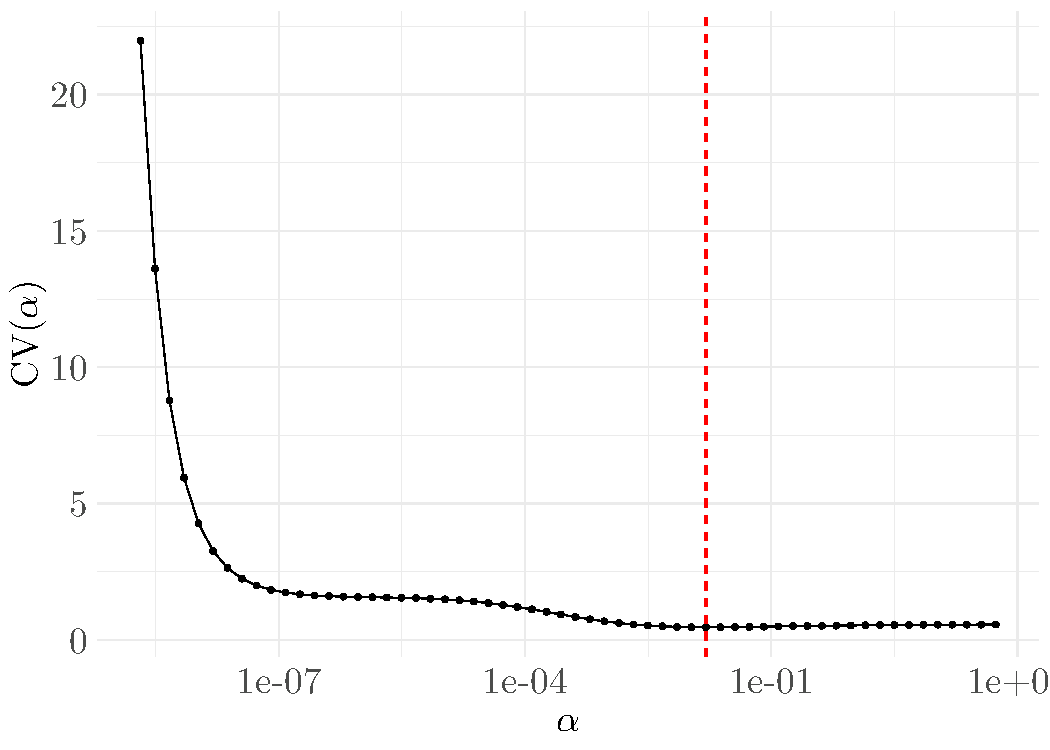
\includegraphics[width=0.45\textwidth]{./figures/notperp/NOTPERP_volume_tikhonov_cv.pdf}\color{black}
	\end{tabular}
	\caption{\small \color{magenta}Cross-validation criteria of the two tuning parameters of the NOTPERP volume application, both on a logarithmic horizontal axis. \textbf{Left:} the design-density criterion, the pointwise median over the $50$ curves on which it is computed, against the bandwidth $h$; the dashed line marks the selected bandwidth $0.005$, which is the lower edge of the grid. \textbf{Right:} the Tikhonov criterion against $\alpha$ over the grid of $60$ points; the dashed line marks the selected $\alpha = 0.016$, which is interior.\color{black}}
	\label{fig:notperp_volume_cv}
\end{figure}

\begin{figure}[h!]
	\centering
	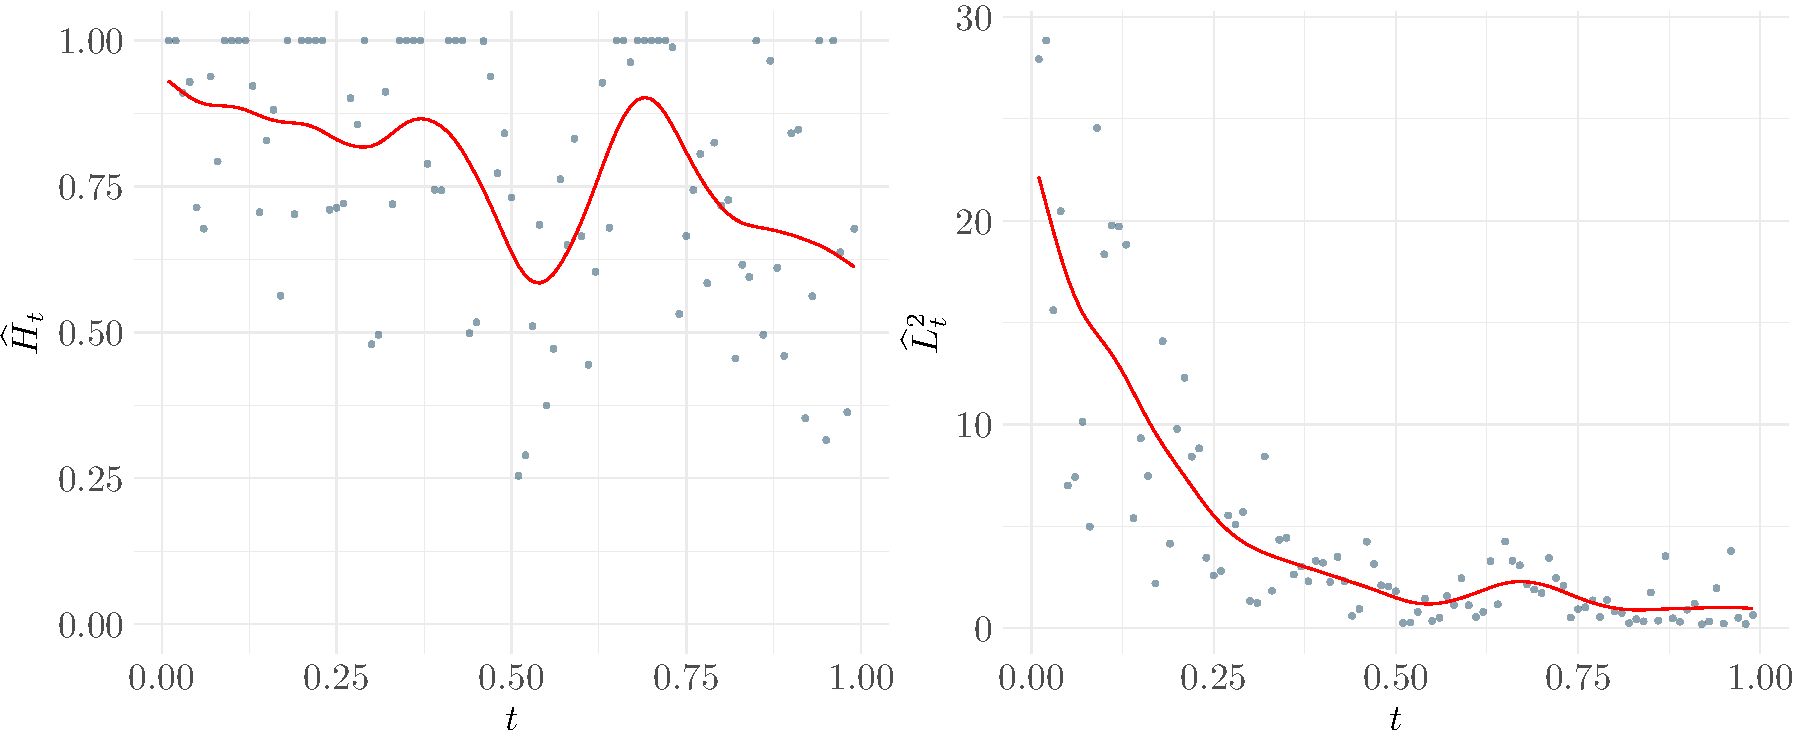
\includegraphics[width=\textwidth]{./figures/notperp/NOTPERP_volume_local_regularity.pdf}
	\caption{\small \color{magenta}Estimated local regularity of the NOTPERP volume curves, at the $99$ equally spaced points $t = 0.01, \ldots, 0.99$. \textbf{Left:} the local Hölder exponent $\widehat{H}_t$, drawn on the whole of the interval $[0,1]$ so that an estimate sitting on the clamp is visible. \textbf{Right:} the local Hölder constant $\widehat{L}^2_t$. In each panel the dots are the pointwise estimates and the solid line a cubic spline smoothing of them.\color{black}}
	\label{fig:notperp_volume_locreg}
\end{figure}

\begin{figure}[h!]
	\centering
	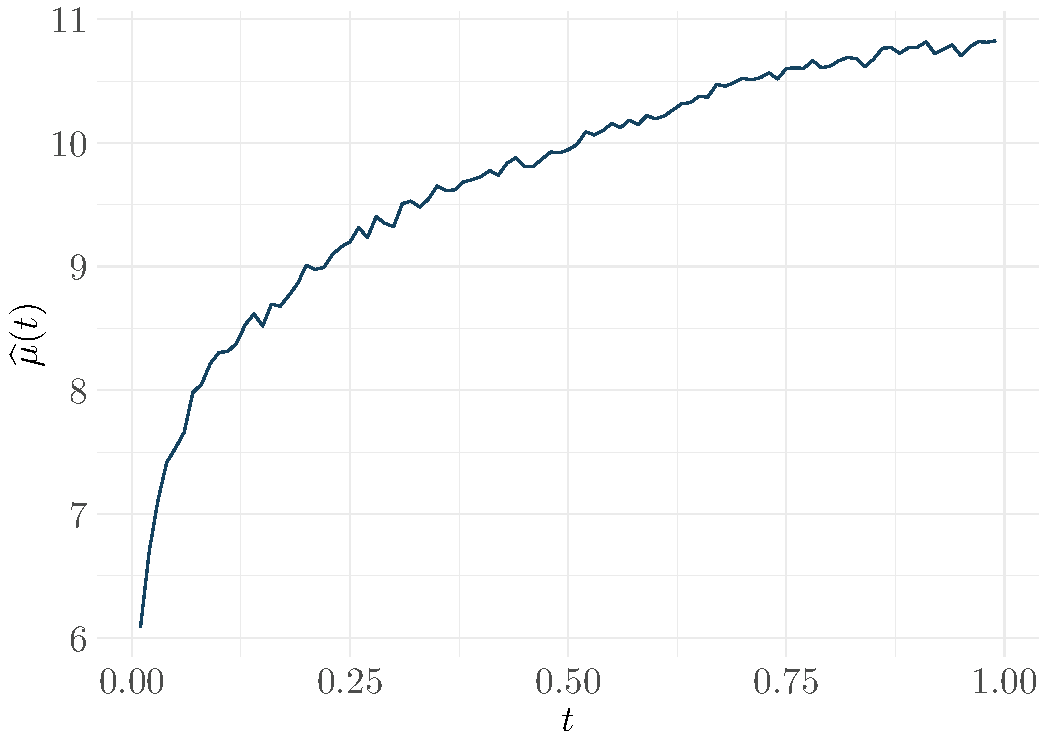
\includegraphics[width=0.7\textwidth]{./figures/notperp/NOTPERP_volume_mean_function.pdf}
	\caption{\small \color{magenta}Estimated mean function $\widehat{\mu}$ of the NOTPERP volume curves, at the $99$ equally spaced points $t = 0.01, \ldots, 0.99$. The response is the logarithm of the notional traded in USDT since midnight UTC, and the horizontal axis is the fraction of the UTC day elapsed.\color{black}}
	\label{fig:notperp_volume_mean}
\end{figure}

\subsubsection{\color{magenta}French electricity production\color{black}}

\color{magenta}
In this section we give more details on the photovoltaic and hydroelectric production curves, which the main manuscript defers. Both are obtained from the ODR\'E platform \citep{odre_data}, both are normalised by dividing every value by the maximum production observed over their period, and both are predicted under the protocol described there for the consumption curves: the last curve of the series is held out entirely, predicted from the one preceding it, and every estimate entering the predictor is computed on the curves before the target. That protocol is not restated here.

Photovoltaic production covers the same period as the consumption curves, 1 June to 30 September 2024, and comprises $122$ daily curves. Output is zero outside daylight, so the curves are restricted to the $61$ quarter-hourly points between 04:00 and 19:00 and their observation times renormalised over the points retained; the design remains common, with $M_n = \lambda = 61$ for every day. The lag-$1$ FACF \eqref{eq:blup:facf} is $0.431$. Figure~\ref{fig:energy_supp_pred} shows the prediction of the last curve of the period, whose values lie in $[0, 0.551]$. The squared error of the prediction, averaged over the $61$ observation points, is $2.411$ times smaller than that of the estimated mean curve, the largest of the three ratios, and the prediction is the closer of the two at every one of the $61$ points. This is likely due to the shape of a solar day being fixed by the sun while only its amplitude varies, so that the lagged curve carries most of what distinguishes one day from the next.

Hydroelectric production comprises $152$ daily curves recorded at $96$ quarter-hourly points between 1 November 2023 and 31 March 2024, taking values in $[0.267, 1]$ over the whole period. The lag-$1$ FACF is $0.365$, the weakest of the three series. The squared error of the prediction is $1.125$ times smaller than that of the estimated mean curve, and the prediction is the closer of the two at $57.3$ per cent of the $96$ points only. Although the gain is slight, it follows the autoregressive effect, which is weakest for this series; this is likely due to hydroelectric output being dispatched against demand and reservoir constraints rather than driven by a physical daily cycle, so that the curve preceding the target constrains it less than in the other two series.

The regularisation parameter is selected by cross-validation for each series over its own grid of $40$ points, each a window of seven to nine natural logarithm units. The default grid of the package selects its own lower boundary on all three series, whose operators are well conditioned and ask for almost no ridge, and above roughly $e^{-5}$ the criterion is flat to four significant figures, so that on a grid wide enough for all three the minimum is compressed into one edge of the picture and cannot be read. Each window is therefore centred on its own minimum. The selection is interior in all three: $2.5\cdot 10^{-5}$ for consumption, $5.7\cdot 10^{-5}$ for photovoltaic and $9.1\cdot 10^{-5}$ for hydroelectric. Figure~\ref{fig:energy_supp_tikhonov} shows the three criteria.
\color{black}

\begin{figure}[h!]
	\centering
	\begin{tabular}{cc}
		\color{magenta}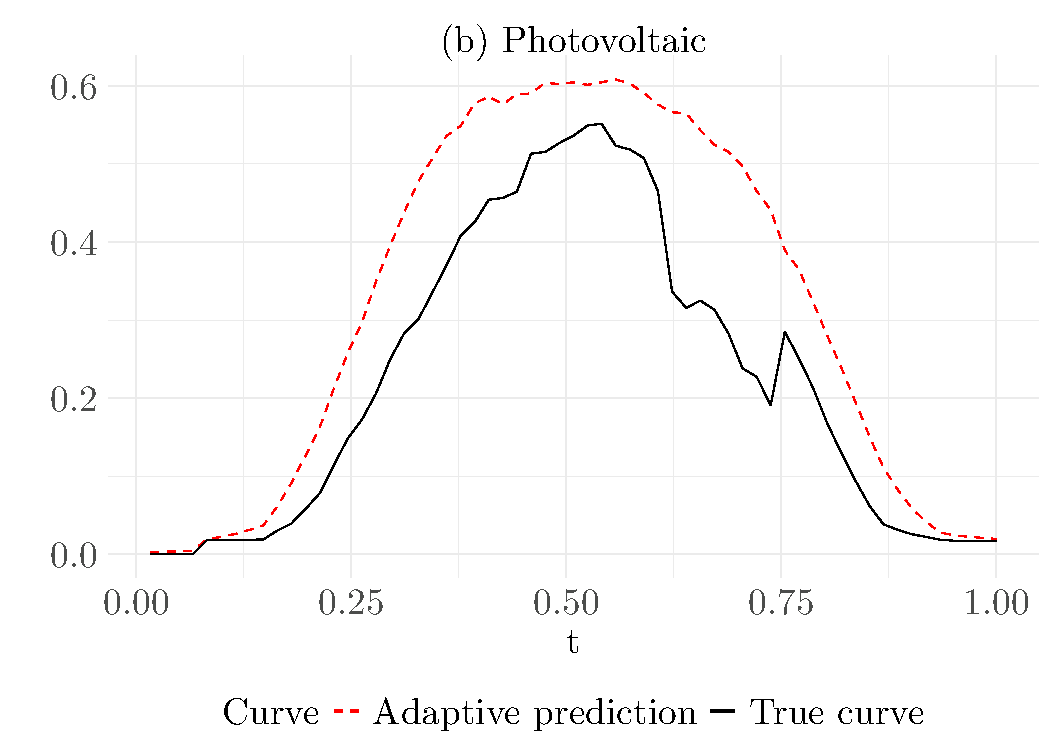
\includegraphics[width=0.45\textwidth]{./figures/blup/plot_adaptive_blup_solaire.pdf}\color{black} &
		\color{magenta}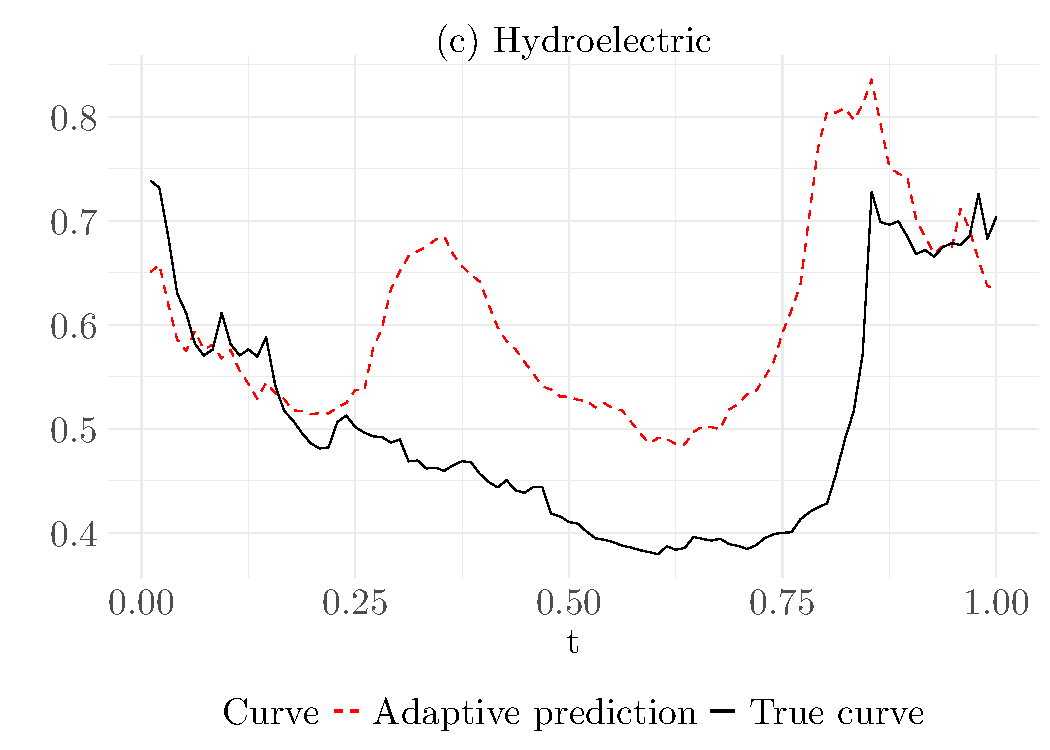
\includegraphics[width=0.45\textwidth]{./figures/blup/plot_adaptive_blup_hydrau.pdf}\color{black}
	\end{tabular}
	\caption{\small \color{magenta}Prediction of the last daily production curve of each series from the curve preceding it. \textbf{Left:} photovoltaic production, at the $61$ quarter-hourly points retained between 04:00 and 19:00. \textbf{Right:} hydroelectric production, at $96$ quarter-hourly points. In each panel the solid line is the observed curve and the dashed line the adaptive prediction, and values are normalised to $[0,1]$ by the maximum production observed over the period.\color{black}}
	\label{fig:energy_supp_pred}
\end{figure}

\begin{figure}[h!]
	\centering
	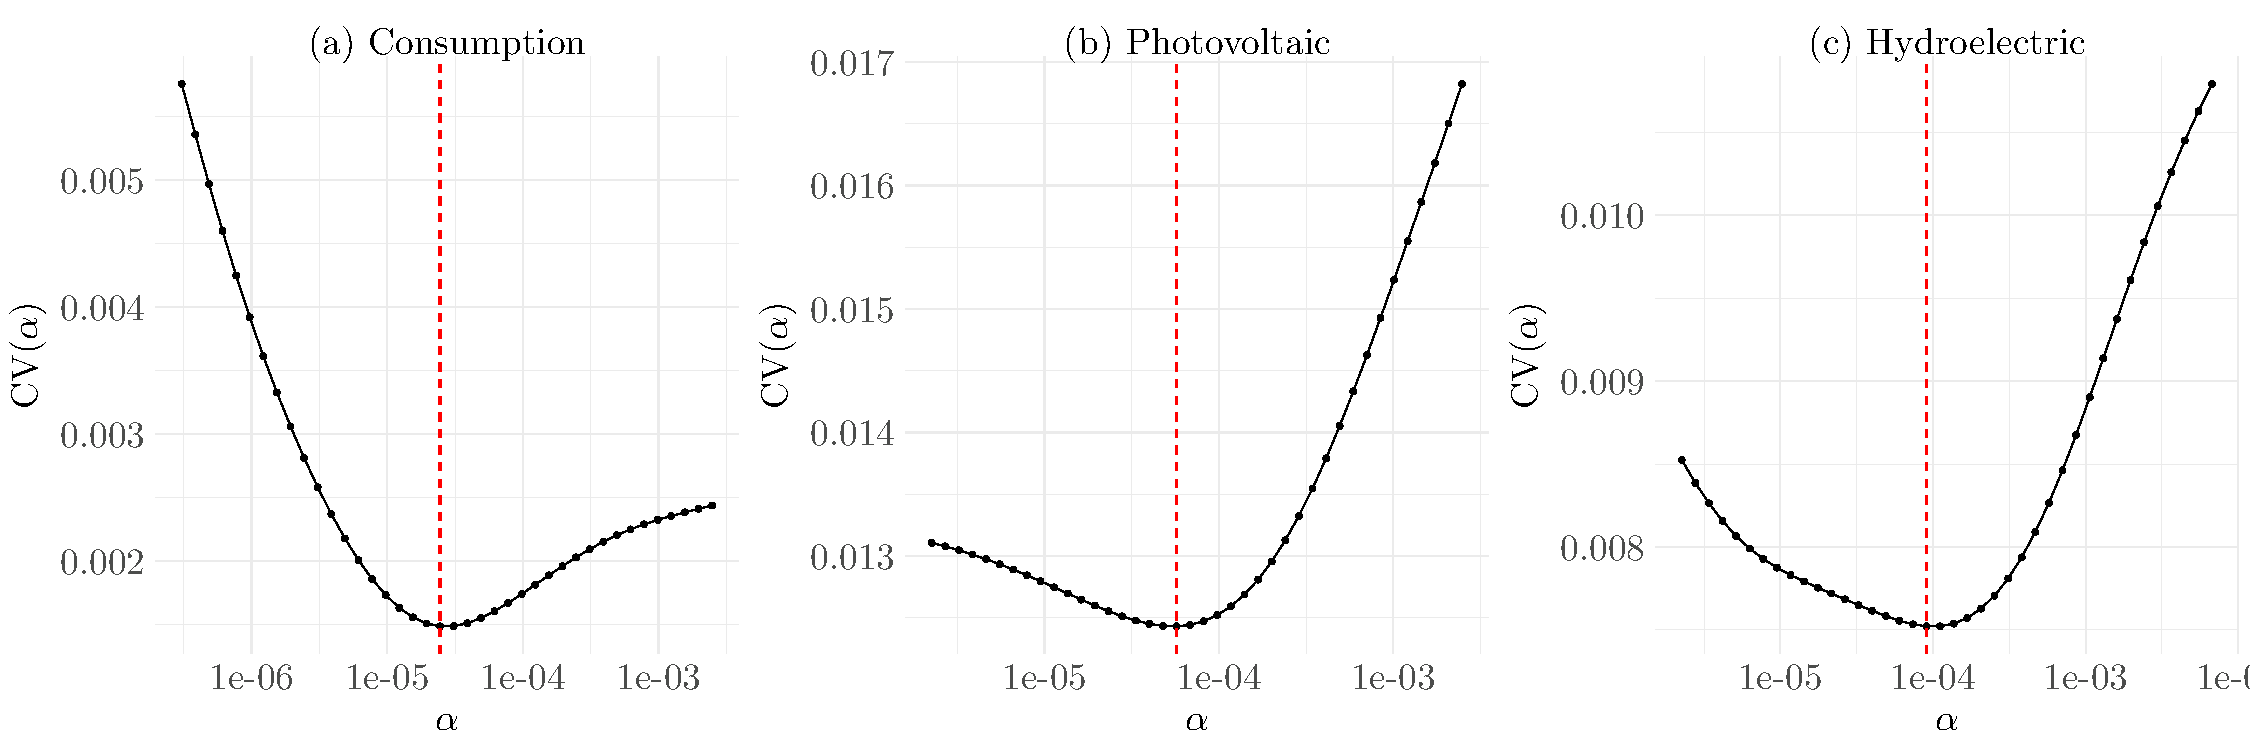
\includegraphics[width=\textwidth]{./figures/blup/plot_tikhonov_cv_energy.pdf}
	\caption{\small \color{magenta}Cross-validation criterion of the Tikhonov parameter for the three electricity series, each over its own grid of $40$ points and on a logarithmic horizontal axis. \textbf{Left:} consumption. \textbf{Middle:} photovoltaic production. \textbf{Right:} hydroelectric production. In each panel the dashed line marks the selected $\alpha$, which is interior to the grid in all three.\color{black}}
	\label{fig:energy_supp_tikhonov}
\end{figure}
